\documentclass[a4paper,10pt]{article}
\usepackage[utf8]{inputenc}
\usepackage{hyperref}
\usepackage{listings}
\usepackage{xcolor}
\lstset { %
    language=C,
    backgroundcolor=\color{black!5}, % set backgroundcolor
    basicstyle=\footnotesize,% basic font setting
}

%opening
\title{Malware}
\author{Guillaume Bonfante}

\usepackage{tikz}

\usetikzlibrary{shapes}
\usetikzlibrary{arrows}
\usetikzlibrary{shadows}
\usetikzlibrary{positioning}

\begin{document}

\maketitle

\section{Introduction}

Securité vs sûreté : \\

La sûreté consiste à vérifier que le système fonctionne correctemenet, tandis que la sécurité introduit le principe d'attaquant, le système fonctionne correctement, mais un attaquant essaye de le détourner.

\paragraph*{}
Cours de 14 séances, les 7 premiers nous allons jouer le rôle des méchants, et les 7 suivants le rôle des gentils.

\paragraph*{}
Les attaques sont fréquentes et ciblent les pays à fort PIB, mais pas seulement. Par exemple, il y a un intérêt à faire du spam, ou des ransomware à des gens choisis dans ces pays. Un autre tye d'attaque moins documenté, sont les attaque étatiques (stuxnet). Un attaque bien connue est WannaCry, car les machines n'étaient pas mise à jour (le responsable informatique souhaitait tout mettre à jour, et le responsable de production a refusé d'arrêter la chaîne poue un ``éventuel problème'', après un calcul de risque ils ont estimé que c'était plus rentable de ne rien arrêter)

\paragraph*{}
Quelques chiffres :
\begin{itemize}
 \item 10 millions : estimation du nombre d'ordinateurs infectés par conficker en 2008 dans plus de 190 pays.
 \item 12 milliards de dollars : coûts estimé des dégâts de Zues en 2010-2012.
 \item 323 000 nouveaux malwares chaque jour en 2016 (selon Kaspersky)
\end{itemize}

\section{Un exemple - Stuxnet}
\begin{center}
  Rapport -- Ralph Langner : ``how to kill a centrifuge''
\end{center}

\paragraph*{}
L'objectif était de ralentir le ncucléaire iranien en attaquant les centrifuges qui enrigissent l'uranium. Quelqu'un s'est introduit sur le site, puis ont localisé tout le matériel, se mettre sur le réseau interne, et enfin attaquer le matériel.

2 scénarios ont été proposé à Obama : un ou on changeait la vitesse des centrifuges pour les faire chauffer et casser, en changeant la valeur des capteurs, ou bien les faire sauter, en augmentant la pression dans certaines gauges.

Pour trouver de l'info sur les virus et des exemples : \url{https://www.botnets.fr/wiki/Main_Page}

\paragraph*{}
Dès qu'une machine lance word, on a tout ce qu'on veut pour faire ce qu'on veut. Word requiert les dll pour dns api, et ncryptssl, ce qui permet de chiffrer une communication entre notre machine et celle-ci.

\section{Un executable}

Un executable est une donnée stockée sur un ordinateur, et se transforme ne executable une fois qu'il est interprêté par un ordinateur.

Un malware est un programme, et de ce fait (théorème, 1940) il ne peut être détecté.

Preuve :
 $P=^?M$ (le programme est un malware, il contient donc exactement les même données que M). Il suffirait donc de vérifier octet par octet qu'ils sont identiques.\\
 En revanche, on a besoin de mieux que ça, on veut que $\left[P\right] =^? \left[M\right]$, c'est à dire que P et M ont les mêmes effets, pas le même code.
\paragraph*{}
 Or, on ne peut pas comparer si deux programmes font exactement la même chose. C'est impossible.

 \section{TP}
 
 On écrit un programme en C pour afficher l'adresse d'une variable qu'on stocke dans la mémoire d'un programme : 
 
\begin{lstlisting}
  #include "stdafx.h"
  
  int _tmain(int argc, _TCHAR* argv[])
 {
    int a = 0x12345678;
    printf("%d\n", & a)
    printf("Hello World");
    while(1);
    return 0;
  }
  
\end{lstlisting}

On va modifier ce snippet pour afficher le contenu en case mémoire et analyser comment sont stockés les ints.

On fait un programme qui va aller lire toutes les cases mémoires le plus loin possible en C (voir VM) : 
\begin{itemize}
 \item La lecture bloque à 0x0041b000.
 \item L'écriture bloque en 0x00405000.
\end{itemize}

La mémoire est découpée en bloc de kilo octets (1000 en hexa).
4 droits, la lecture, l'écriture, executer (il y a des cases executables ou non executables, et finalement le dernier, le droit de l'administrateur (toutes celles qui vont toucher le materiel, interdites pour un utilisateur normal).


Sur windows, tous les executables commencent par MZ, on dit que c'est le header.
\begin{center}
 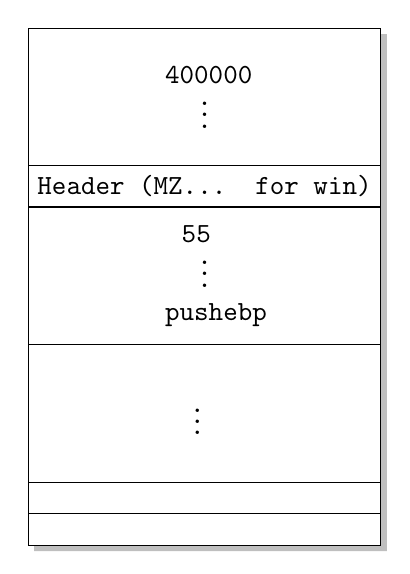
\begin{tikzpicture} [
            % ----- Node definitions ----- %
            dirtablenode/.style = {
                    draw,
                rectangle, 
                rectangle split,
                rectangle split parts = #1,
                fill = white!5,
                align=center,
                drop shadow,
                font=\ttfamily
            },
    ]
    
            % ----- Node constructions ----- %
        \node [dirtablenode=6] (directory) {
            \nodepart{one}
                \parbox[t][15mm][c]{1cm}{400000 \\ \centering \vdots}
            \nodepart[]{two}   
                Header (MZ... for win)
            \nodepart{three} 
		\parbox[t][15mm][c]{1cm}{55\\ \centering \vdots \\ pushebp}
            \nodepart{four} 
                \parbox[t][15mm][c]{1cm}{\vdots}
        };
          
\end{tikzpicture}


\end{center}

Tous les programmes ont donc une structure comme celle ci : 


\begin{center}
 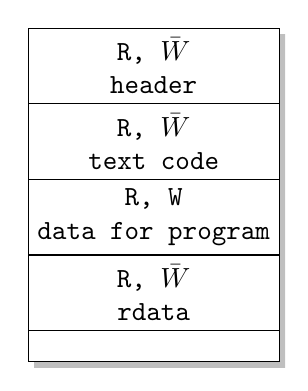
\begin{tikzpicture} [
            % ----- Node definitions ----- %
            dirtablenode/.style = {
                    draw,
                rectangle, 
                rectangle split,
                rectangle split parts = #1,
                fill = white!5,
                align=center,
                drop shadow,
                font=\ttfamily
            },
    ]
    
            % ----- Node constructions ----- %
        \node [dirtablenode=5] (directory) {
            \nodepart[]{one}
                R, $\bar{W}$ \\ header
            \nodepart[]{two}   
		R, $\bar{W}$ \\ text code
            \nodepart[]{three} 
		R, W \\data for program
            \nodepart[]{four} 
		R, $\bar{W}$ \\rdata
        };
          
\end{tikzpicture}
\end{center}

Le Header fait en réalité 1000 Ko, et seuelement 200Ko sont réellement utilisés, on peuut écrire environ n'importe quoi dedans.

\paragraph*{}
On peut lire les octets des fonctions aussi : 

\begin{lstlisting}
#include "stdafx.h"
  
  int _tmain(int argc, _TCHAR* argv[])
 {
    char* q = (char*) printf;
    printf("%x\n", q[0])
    printf("Hello World");
    while(1);
    return 0;
  }
 
\end{lstlisting}

Ce petit programme nous permet de voir que printf commence par 6a. En particulier, on peut aussi afficher la meme chose pour des fonctions donnant des autorisations de modifications de fichier, par exemple virtual mem protect. 

\paragraph*{}
Le ``jeu'' pour un hacker est de cacher les appels fait aux fonctions systèmes pour pas qu'on voit l'execution du programme. 
Pourquoi ? Car sur IDA (voir VM), on peut analyser l'executable et voir les fonctions systèmes auxquels le programme fait appel. Si une image fait appel à l'api dns, c'est pas trop normal par exemple, et toutes ces fonctions sont écrites au début.

\begin{figure}[h!]
 \centering	
 \includegraphics[width=\textwidth]{malware/ida}
 \caption{Disassembly with ida}
\end{figure}

La solution est de se débarasser de printf en cherchant son pointeur d'instruction et en accédant au code de la fonction.

\begin{lstlisting}
#include "stdafx.h"
  
  int _tmain(int argc, _TCHAR* argv[])
 {
    char* p = (char*) scanf;
    char* q = (char*) printf;
    printf("%p %p", p, q)
    while(1);
    return 0;
  }
 
\end{lstlisting}

L'écart entre les deux est de 1200, printf = scanf - 1200.
On enlève alors la ref à printf et on la remplace par scanf - 1200, puis on va bouger le pointeur de fonction pour executer les instructions présente à p.

\begin{lstlisting}
#include "stdafx.h"
//structure de la fonction printf : 
typdef vois (type_function)(const char *, ...); 

  int _tmain(int argc, _TCHAR* argv[])
 {
    char* p = (char*) scanf;
    char* q = p - 1200;
    type_function f;
    f = (type_function) p;
    f("Hello World");
    while(1);
    return 0;
  }
 
\end{lstlisting}

\section{Instructions en assembleur}

\subsection{Les registres}

Les registres de stockage sont :
\begin{itemize}
 \item EAX
 \item EBX
 \item ECX
 \item EDX
\end{itemize}

Ceux pour stocker les chaines de charactères : 
\begin{itemize}
 \item ESI
 \item EDI
\end{itemize}

Ceux pour la pile et les arguments de la fonction en cours : 
\begin{itemize}
 \item ESP (pile)
 \item EBP (arguments)
\end{itemize}

Le pointeur d'instruction : 
\begin{itemize}
 \item EIP (or RIP), on en peut pas faire un mov dessus, c'est interdit.
\end{itemize}

Les registres historiques : 
\begin{itemize}
 \item CS, DS, ES, FS (L'OS utilise ce registre pour stocker des infos), GS, SS
\end{itemize}

Voir ensuite les \href{https://en.wikipedia.org/wiki/Control_register}{Control Registers}	for OS processor.

\paragraph*{}
Il est extremement difficile d'obtenir la liste des instructions x64 processeur, certains projets essayent cependant d'en établir une liste. Les projets open source \href{http://www.capstone-engine.org/}{Capstone} et \href{https://github.com/zyantific/zydis}{Zydis} par exemple.

\subsection{L'assembleur}
\begin{lstlisting}
 mov eax, ebx             ; eax = ebx
 mov eax, 0x1234          ; eax = 0x1234
 mov eax, [ebx]           ; eax = ebx
 mov eax, dword ptr [ebx]
 mov eax, [ebx + 4*ecx]   ; eax = ebx[ecx]
 mov eax, fs:[0x30]          ; eas = fs[30]
\end{lstlisting}
NB : sur cette avant dernière instruction, on peut avoir un 1*, 2*, ou 4*.

\paragraph*{}
\begin{lstlisting}
 mov [eax], ebx
 mov [eax] 0x1234
 mov [eax], [ebx]
\end{lstlisting}

Cette dernière instruction n'est pas de l'assembleur, elle existe en MASM (asm microsoft) mais elle est simplement recompilée en  instructions élémentaires.

Pour mettre à zero un registre :
\begin{lstlisting}
 xor eax, eax
\end{lstlisting}

\paragraph*{}
Pour déplacer le pointeur d'instruction :
\begin{lstlisting}
 jmp 0x4000 000 ; EIP = 0x400 000
 jmp [0x1234]   ; EIP = *(0x1234)
 jmp eax
\end{lstlisting}

Les deux ernières instructions sont des cauchemards pour retracer où le pointeur d'instruction va, et pourtant elles sont présentes dans quasi tous les executables.

Exemple : 
On souhaite appeler printf, qui n'est pas présent dans notre cote (sur windows il est dans une dll) dans l'executable, on a alors stocké quelque part l'adresse de printf dans une case mémoire. tous les appels à printf sont alors compilés par des jumps à cette adresse là.

\paragraph*{}
Il y a toute une liste d'instructions de jump conditionnels (voir slides ou en ligne). 

\subsection{Un appel de fonction}

On appelle ici la fonction dont l'adresse est stockée en 1234 : 
\begin{lstlisting}
 push eax
 push 0x1234
 pop eax  ; dépile et stock le res dans eax
 call [0x1234] ; or call eax
\end{lstlisting}

\section{Code obfuscation}

On veut obfusquer le code suivant : 

\begin{lstlisting}
#include "stdafx.h"
char chaine [] = "Hello world";

  int _tmain(int argc, _TCHAR* argv[])
 {
    printf(chaine)
    while(1);
    return 0;
  }
 
\end{lstlisting}

On utiliise un opérateur idempotent (XOR) pour chiffrer le hello world : 

\begin{lstlisting}
#include "stdafx.h"
char chaine [] = "Hello world";

  int _tmain(int argc, _TCHAR* argv[])
 {
    for (int i=0, i < 12; ++i) {
      print("\\x%02x", chaine[i] ^ 0x42);
    }
    while(1);
    return 0;
  }
 
\end{lstlisting}

Le programme sort alors le résultat suivant : 
\begin{lstlisting}
 \x0a\x27\x2e\x2e\x2d\x62\x35\x2d\x30\x2e\x26\x42
\end{lstlisting}

On modifie alors notre code afin que le hello world soit totalement caché : 

\begin{lstlisting}
#include "stdafx.h"
char chaine [] = "\x0a\x27\x2e\x2e\x2d\x62\x35\x2d\x30\x2e\x26\x42";

  int _tmain(int argc, _TCHAR* argv[])
 {
    for (int i=0, i < 12; ++i) {
	  chaine[i] = chaine[i] ^ 0x42;
	}    
    print(chaine);
    while(1);
    return 0;
  }
 
\end{lstlisting}

Un exemple de programme assembleur MASM pour faire un simple print : 

\begin{lstlisting}
#include "stdafx.h"

  int _tmain(int argc, _TCHAR* argv[])
 {
    char * format = "%s";
    char * hello = "Hello World !"
    __asm {
      mov eax, [hello]
      push eax
      mov eax, [format]
      push eax
      call dword ptr(printf)
      pop eax
      pop eax
    }
    while(1);
    return 0;
  }
 
\end{lstlisting}

Maintenant, essayons d'utiliser la chaine de charactère cryptée de tout à l'heure.	


\begin{lstlisting}
#include "stdafx.h"

  int _tmain(int argc, _TCHAR* argv[])
 {
    char [] format = "%s";
    char [] chaine = "\x0a\x27\x2e\x2e\x2d\x62\x35\x2d\x30\x2e\x26\x42"
    __asm {
      mov edx, 12 ; loop counter
  debut: 
      lea eax, [chaine]
      mov ebx, 0x42
      xor [eax + edx], bl
      dec edx
      cmp edx, -1
      jnz debut
  funcall:
      push eax
      lea eax, [format]
      push eax
      call dword ptr(printf)
      pop eax
      pop eax
    }
    while(1);
    return 0;
  }
 
\end{lstlisting}

NB: on peut utiliser lea avec crochets pour les char [] ou bien mov avec les crochets pour un char*.

\section{Structure d'un executable, et d'un process dans la mémoire}

En 1970, la mémoire coûte cher, donc dès qu'on peut faire des cut on va les faire, donc les processus stockent un poil moins d'info que les executables. Lorsqu'on écrit un code, on a accès à toutes les fonctions du processus en faisant : 
\begin{lstlisting}
  #include <windows.h>
\end{lstlisting}

\subsection{Structure d'un executable}

NB: tous les executables windows commencent par NZ, et donc lorsqu'on copy paste un virus sur notre desktop, il se fera supprimer, mais si on change le NZ par PY par exemple, vu que le fichier n'est plus executable, windows n'a aucune raison de le considérer comme une menace.

On peut utiliser la commande hexdump pour regarder la structure binaire du fichier.

Après les headers, on le DOS header contenant : 
\begin{itemize}
 \item Machine, i.e x86 ou x64, si ça a été compilé pour 3 ou 64 bits
 \item Le nombre de sections (de codes et de data) c'est à dire .text, .data et .resource pour un fichier assembleur.
 \item Des Caractéristiques, i.e si on est en mode debug ou si on est une dll.
\end{itemize}

Dans le optional header, il y a beaucoup plus de choses (voir slides), parmi ceux ci les plus utiles
\begin{itemize}
 \item La taille du code mis en mémoire, information qu'on peut employer
 \item La taille des données initialisées au préalable (typiquement taille de la section .data) et la taille des données non initialisée.
 \item Le point d'entrée du code
 \item Image base, qui est la position en mémoire de l'executable (la position que le programme demande au système, par défaut, pour s'executer, qui est en général acceptée par le système, typiquement sur windows c'est un 400 000 et quelques)
 \item La taille en mémoire de l'executable, et typiquement avec la Image base et la taille de l'executable, vous avez exactement la part de mémoire qui va être utilisée par le mémoire. À cet endroit là, il peut demander manuellement l'allocation de sa pile (par exemple, s'il a besoin de 3Go de ram, il peut le demander ici)
\end{itemize}

Toute cette section se termine par 16 tables, dont 2 importantes.
La export table, dans laquelle on inique quelles sont les fonctions dans l'executable. Dans un executable normal, il y a juste main, et pour une DLL, il y a toutes les fonctions de la dll (une api). Lorsqu'on veut executer printf, on peut appeler la dll qui contient printf, dans laquelle on aura l'adresse de la fonction.

La seconde est la talbe d'import, qui fait l'opération inverse, qui indique pour un programme donné, la liste des dll qu'il utilise, et la liste des fonctions qu'il emploie dans ces dll. C'est pour cette raison là qu'on aperçoit rapidement quand on utilisait printf. C'est un méchanisme difficile à contourner.

\paragraph*{}
De nombreux antivirus utilisent cette table pour detecter les virus.

\paragraph*{}
Experience Bonfante : Prendre mediacrypt, et remplacer le code par des zeros, mais garder la table d'import. Plein d'antivirus vont reconnaître médiacrypt. de fil en aiguille on peut voir de quels éléments dépendent leur signature, et pour plein, c'est uniquement la table d'import.

\paragraph*{}
D'autres tables moins importantes, une pour les certifications, une pour déplacer l'executable dans la mémoire, etc...

\subsubsection{Détails sur la table d'export}
La table d'export est une structure windows, dans laquelle on retrouve le nom de la dll, et son nom en version courte. Le nombre de fonctions, leur nom ou numéro, et trois tables qui correspondent aux adresses des fonctions. Ces addresses là seront déterminées à l'execution, c'est la SEULE partie qui sera modifiée par le système, à l'execution.

\subsubsection{Détails sur la table des sections}
Cette table a la même taille que le nombre de sections (c'est pourquoi le nombre de section est hardcodé plus haut, pour retrouvé la taille de cette table). S'il y a une section .rdata (readonly) c'est à cet endroit qu'on va voir les autorisations dessus et donc qu'elle est readonly.
\paragraph*{}
Donc il suffit juste de changer cette table pour dire tiens je veux écrire dans la section rdata, et tout d'un coup ça devient autorisé, et le programme peut écrire dans cette section alors qu'il n'avait pas le droit.

\paragraph*{}
Dans cette table il y a aussi le nom de la section, la taille de la section, la position en mémoire, et finalement les droits en mémoire mentionnés plus haut. Dans les sections principales, on trouve la section text qui est le code (microsoft s'attend à ce que le premier appel soit dans la seciotn text, même si ce n'est pas obligatoire).

\subsection{TP}
Une autre manière de retrouver printf, est de désassembler un executable dans lequel on appelle printf, et de regarder la table d'import dans IDA. On a ainsi accès à la DLL dans laquelle est stockée la fonction printf (en bas dans la photo suivante).


\begin{figure}[h!]
 \centering	
 \includegraphics[width=\textwidth]{malware/ida-import}
 \caption{Table d'import}
\end{figure}
Il y en a beaucoup qui sont là à cause du mode debug, en mode release, on en aurait que 2.

\paragraph*{}
Exemple de récupération de fonction via une dll:
\begin{lstlisting}
 #include "stdafx.h"
 #include <Windows.h>

typdef int (type_function)(const char *, ...);
int _tmain(int argc, _TCHAR* argv[])
{
  HMODULE msvcr = LoadLibrary(L"MSVCR100D.dll");
  type_function fonction = (type_function) GetProcAddress(msvcr, "printf");
  fonction("Hello World");
  while(1);
  return 0;
}
  
 
\end{lstlisting}

Ici, on ne voit pas printf dans la table d'import (dans ce cas là, on le verra en string, mais on a vu qu'on pouvait le crypter sans pb).

Bien évidemment, si on a seulement deux imports dans un executable, l'antivirus va détecter l'executable comme étant un ``malware générique`` car il n'y aura pas assez d'appel à des libraries.

\paragraph*{}
Typiquement dans un malware, les apels cachés comme on a fait sont surtout utilisés pour récupérer GetProcAddress et cacher les récupérations de toutes les fonctions. 

\subsection{Execution de données, et automodification de code}

\subsubsection{Execution de données}

On souhaite ici executer une instruction stockée dans une variable. Ici, on exploite le fait qu'en hexa l'instruction nop est codée par $90$ en hexa. Dans le programme suivant, on stocke cette instruction sous forme de string pour l'executer ensuite.

\begin{lstlisting}
 #include "stdafx.h"
 #include "string.h"

char code [] = {'\x90', '\x90', '\x90'}

typdef void (*fonction_vide)();

int _tmain(int argc, _TCHAR* argv[])
{
  fonction_vide fonction = (fonction_vide) (& code);
  fonction();
  while(1);
  return 0;
}
  
 
\end{lstlisting}

Lorsqu'on execute cette fonction, elle plante, car la liste de char qu'on a mis ne peut pas être codée sur 3 octets pour 3 chars, et lorsque le compilo tourne, en initialisant les variables, il initialise les char avec une liste de zéro à la fin qui en assembleur l'instruction GetPointer, ce qui va tout faire planter.

Variable char code: \\ \vspace{5mm}

 \begin{center}
\begin{tabular}{ |c|c|c|c|c|c|c|c|}
\hline
 $\backslash x90 $& $\backslash x90 $& $\backslash x90 $& 0 & 0 & 0 & 0 & 0\\ 
\hline
\end{tabular}
\end{center}


Comme on a manuellement hardcodé ces instructions pour être dans une fonction, en fait en débuggant, en mettant un breakpoint et en executant puis un petit click droit afficher le code machine, on peut voir que les nops sont executés, seulement ça plante quand ç aexecute les zéros. Que mettre à la fin d'une fonction en assembleur pour qu'une fonction ne plante pas, ou alors n'execute pas ces zéros ? un ret.

On change alors le code précédant pour ajouter un ret à la fin de notre tableau d'instruction, le ret est codé en hexa par un $\backslash xc3$. Ainsi, il suffit de stocker dans le char code la même chose avec un $\backslash xc3$ à la fin, qui arrivera avant les zeros.

 \begin{center}
\begin{tabular}{ |c|c|c|c|c|c|c|c|}
\hline
 $\backslash x90 $& $\backslash x90 $& $\backslash x90 $& $\backslash xc3$ & 0 & 0 & 0 & 0\\ 
\hline
\end{tabular}
\end{center}

Il suffit alors de modifier la ligne :

\begin{lstlisting}
 char code [] = {'\x90', '\x90', '\x90'}
\end{lstlisting}

Par : 


\begin{lstlisting}
 char code [] = {'\x90', '\x90', '\x90', '\xc3'}
\end{lstlisting}

Maintenant, le code compile sans problème.

\subsection{Code automodification}
Maintenant, on souhaite faire un code qui se modifie en s'executant, pour se faire on va stocker la fonction \_tmain dans une variable et modifier son contenu comme on vient de le faire.

\begin{lstlisting}
 #include "stdafx.h"
 #include "string.h"

char code [] = {'\x90', '\x90', '\x90'}
char code2 [] = {'\xb6', '\x42', '\x00', '\x00', '\x00', '\xc3'}

typdef void (*fonction_vide)();
typedef int (*fonction_int) ()

int _tmain(int argc, _TCHAR* argv[])
{
  fonction_vide fonction = (fonction_vide) (& code);
  int i = fonction(); \\ executes the nop
  fonction_int f = (fonction_vide) (&code2);
  
  printf("%d\n", i);
  char * p = char * _tmain;
  
  f = (function_int) _tmain
  while(1);
  return 0;
}
\end{lstlisting}

Ce code ne tourne pas car on a vu qu'une section de code n'était pas modifiable une fois compilée. Une première solution serait de modifier dans le header du fichier (voir partie 7) dans la table des sections, mais les anti-virus repèrent ça de suite. Nous pouvons cepandant utiliser une fonction windows faite pour nous : \texttt{VirtualProtect}.

\end{document}
